\documentclass[11pt, oneside]{article} 
\usepackage{geometry}
\geometry{letterpaper} 
\usepackage{graphicx}
	
\usepackage{amssymb}
\usepackage{amsmath}
\usepackage{parskip}
\usepackage{color}
\usepackage{hyperref}

\graphicspath{{/Users/telliott_admin/Dropbox/Tex/png/}}
% \begin{center} 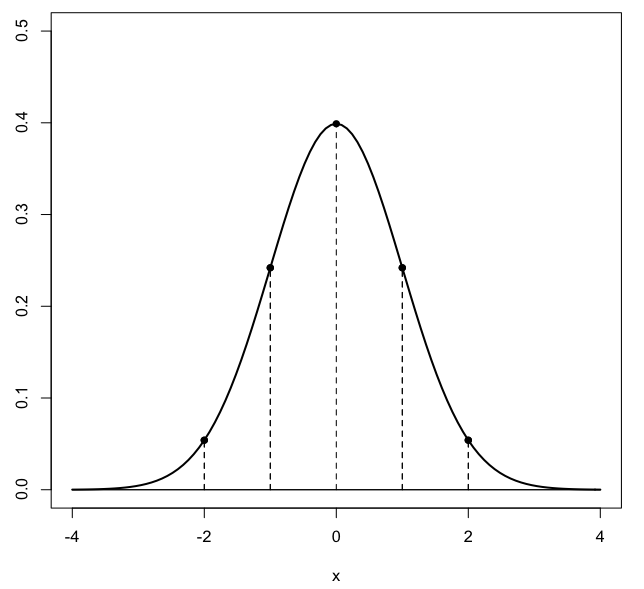
\includegraphics [scale=0.4] {gauss3.png} \end{center}

\title{Sum of angles:  sine}
\date{}

\begin{document}
\maketitle
\Large
Our goal here is to extend the result for the cosine of the sum of two angles to the sine.  My favorite geometric proof of the former is from Strang.  
\begin{center} 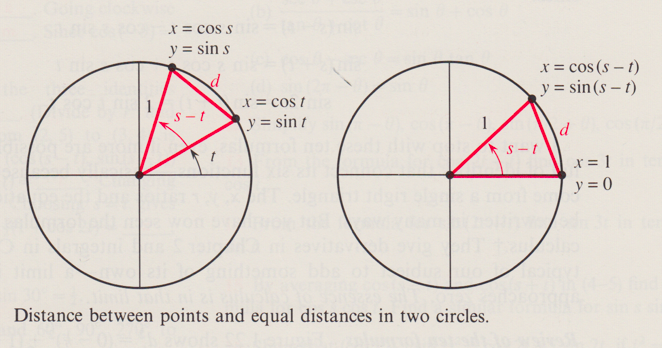
\includegraphics [scale=0.4] {strang_sum.png} \end{center}
The result is
\[ \cos s - t = \cos s \cos t + \sin s \sin t \]
I find this easy to remember because it can be checked for the case $s=t$ so the left-hand side is clearly equal to $1$ and the right-hand side is a well-known identity.  Writing the equivalent formula for the addition $s + t$ is a simple matter:
\[ \cos s - (-u) = \cos s \cos -u + \sin s \sin -u \]
\[ \cos s + u = \cos s \cos u - \sin s \sin -u \]

The next question is often a stumbling block---how to extend the result to the sine?

At this point, we look at the relationships between sine and cosine for angles that are related by addition or subtraction of $\pi/2$.
\begin{center} 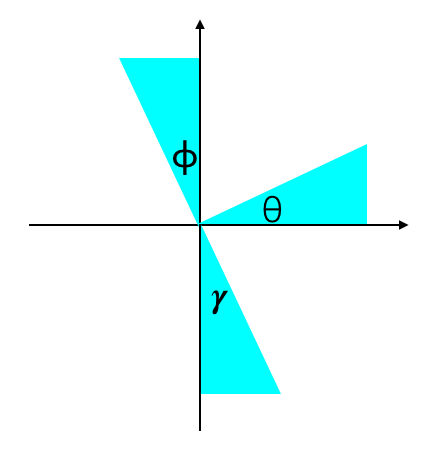
\includegraphics [scale=0.4] {angles.png} \end{center}
In the figure, I have simply rotated the same triangle.  The angle $\phi = \theta$, but what we're really interested is the angle formed with the positive $x$-axis, which we will call $\theta + \pi/2$.

From the figure we can easily read off these four identities
\[ \sin (\theta + \pi/2) = \cos \theta \]
\[ \cos (\theta + \pi/2) = -\sin \theta \]
And
\[ \sin (\theta - \pi/2) = -\cos \theta \]
\[ \cos (\theta - \pi/2) = \sin \theta \]

Now, to solve our problem use the second one above to write
\[ \sin \theta = -\cos (\theta + \pi/2) \]
\[ \sin s + t = - \ [ \ \cos (s + t + \pi/2) \ ]  \]
\[ \sin s + t = - \ [ \ \cos (s + (t + \pi/2)) \ ]  \]
\[ \sin s + t = - \ [ \ \cos s \cos (t + \pi/2) - \sin s \sin (t +  \pi/2) \ ] \]

We can also rewrite the terms:
\[ \cos (t + \pi/2) = -\sin t \]
\[ \sin (t + \pi/2) = \cos t \]
substitute into
\[ \sin s + t = - \ [ \ \cos s \cos (t + \pi/2) - \sin s \sin (t +  \pi/2) \ ] \]
\[ = - \ [ \ \cos s (-\sin t ) - \sin s \cos t \ ] \]
\[ = \sin s \cos t + \cos s \sin t  \]


\end{document}